\frame{\frametitle{Job-B"orse}%Ziel: entwicklung von Anwendungen zur freien und unabhängigen benutzung durch Analphabeten
	\begin{center}
		"Text-freie Benutzereingabe für Analphabeten und semi-gebildete Benutzer"\\
		\vspace*{0.5cm}
		Indrani Medhi, Aman Sagar und Kentaro Toyama\\
	\end{center}
	2006
}
\frame{\frametitle{Testpersonen}
	60 Personen aus 3 Urban-Slums in Indien:\\
	\begin{itemize}
		\item Muttersprache meist Kannada
		\item meist Analphabeten
		\item keine Erfahrung mit Computer
		\item Berufsspanne:
		\begin{itemize}
			\item Haushälter/in
			\item Hausmeister
			\item Bauarbeiter
			\item ...
		\end{itemize}
	\end{itemize}
}

\frame{\frametitle{Designschlüsse}
	\begin{itemize}
		\item vermeiden von Text
		\item Nummern sind verständlich
		\item Audioausgabe
		\item Hilfe anbieten
		\item Bilder verwenden
		\item Kultur berücksichtigen 
		\item höherer Detailgrad bei Zeichnungen
	\end{itemize}
}
\frame{\frametitle{Kulturfehler}
	\begin{figure}
		\centering
		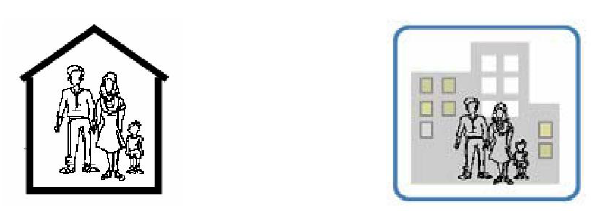
\includegraphics[width=\textheight]{Slides/Design_Anforderungen/Daten/town.PNG}
	\end{figure}
}
\frame{\frametitle{Detailfehler}
	\begin{figure}
		\centering
		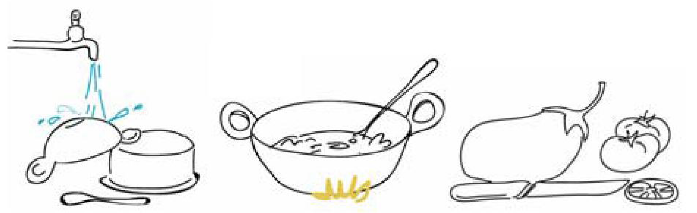
\includegraphics[width=\textheight]{Slides/Design_Anforderungen/Daten/verb-fehler.PNG}
	\end{figure}
}
	\frame{\frametitle{Prototyp-Map}
		\begin{figure}
			\centering
			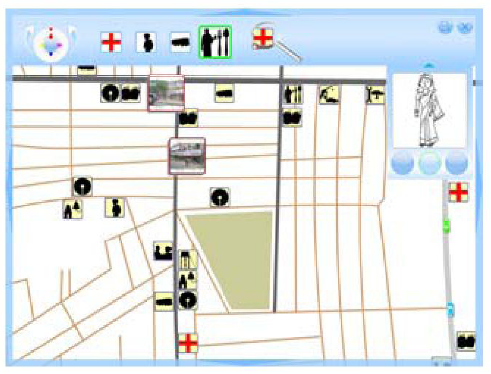
\includegraphics[width=\textheight]{Slides/Design_Anforderungen/Daten/map.PNG}
		\end{figure}
	}
	\frame{\frametitle{Prototyp-Auswahl}
		\begin{figure}
			\centering
			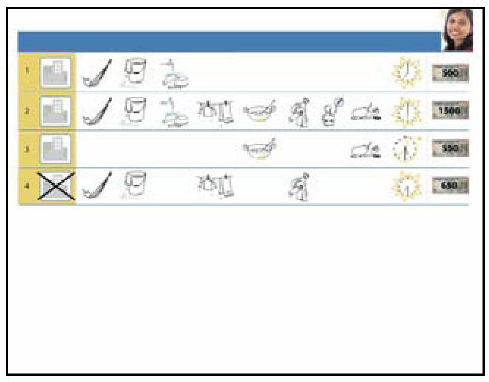
\includegraphics[width=\textheight]{Slides/Design_Anforderungen/Daten/joblist.PNG}
		\end{figure}
	}
	\frame{\frametitle{Prototyp-Job}
		\begin{figure}
			\centering
			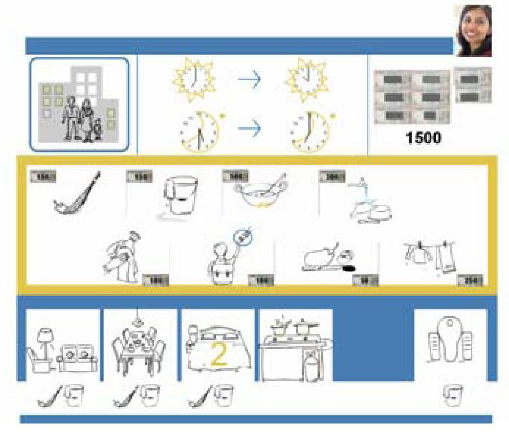
\includegraphics[width=\textheight]{Slides/Design_Anforderungen/Daten/job.PNG}
		\end{figure}
	}

	\frame{\frametitle{Test}
		 Getestet wurden:\\
		\begin{itemize}
			\item Prototyp mit Hilfe
			\item Prototyp ohne Hilfe
			\item Herkömmliche Anwendung mit identischen Inhalt
		\end{itemize}\pause
	\vspace*{0.5cm}
		\begin{itemize}
			\item Ist die herkömmliche Anwendung zug"anglich für die Testgruppe?
			\item Sind die Designschlüsse ausreichend für die Testgruppe?
			\item Welche Anwendung ist am zug"angiger?
		\end{itemize}
	}
	% herkömmliche Anwendung ist nicht anwendbar
	% funktionsweise schnell erkannt, inhalt unschlüssig
	% voice feedback ist "funny" und hilfreich
	% benutzer gruppen kahmen besser zurecht
	% hilfe beruhigt und bechleunigt anwendung
	% navigation wie ein buch zugänglicher